\documentclass[11pt]{article}
\newcommand{\ReportDate}{2 October 2026}
% Preamble for the roughness technical report. Numbers are NOT typed here:
% they come from ../build/numbers.tex, generated by src/build_report.py.
\usepackage[T1]{fontenc}
\usepackage[utf8]{inputenc}
\usepackage{lmodern}
\usepackage[scaled=0.92]{helvet}
\usepackage[letterpaper,margin=1in,headheight=14pt]{geometry}
\usepackage{microtype}
\usepackage{amsmath}
\usepackage{graphicx}
\usepackage{booktabs,tabularx,array,makecell,longtable,threeparttable}
\usepackage[per-mode=symbol,detect-all]{siunitx}
\usepackage[table]{xcolor}
\usepackage[font=small,labelfont=bf,labelsep=period,justification=raggedright,singlelinecheck=false]{caption}
\usepackage{subcaption}
\usepackage{enumitem}
\usepackage{float}
\usepackage{placeins}
\usepackage{fancyhdr}
\usepackage[nobottomtitles*]{titlesec}
\renewcommand{\bottomtitlespace}{0.12\textheight}
\usepackage{textcomp}
\usepackage{tikz}
\usetikzlibrary{positioning,arrows.meta}
\usepackage[hidelinks]{hyperref}
\hypersetup{pdfauthor={Stephen Eacuello}}
\widowpenalty=10000 \clubpenalty=10000
\hyphenation{time-stamps}

\definecolor{ink}{HTML}{0B0B0B}
\definecolor{ink2}{HTML}{52514E}
\definecolor{rule}{HTML}{C9C8C2}
\definecolor{navy}{HTML}{002147}
\definecolor{note}{HTML}{F4F3EF}
\definecolor{gold}{HTML}{B8860B}

\sisetup{group-minimum-digits=5, round-mode=none}
\setlist{nosep, leftmargin=1.4em}
\setlength{\parskip}{0.45em}
\setlength{\parindent}{0pt}
\renewcommand{\arraystretch}{1.12}

\titleformat{\section}{\normalfont\sffamily\Large\bfseries\color{navy}}{\thesection}{0.6em}{}
\titleformat{\subsection}{\normalfont\sffamily\large\bfseries\color{navy}}{\thesubsection}{0.6em}{}
\titleformat{\subsubsection}{\normalfont\sffamily\normalsize\bfseries}{\thesubsubsection}{0.6em}{}
\titlespacing*{\section}{0pt}{1.2em}{0.5em}
\titlespacing*{\subsection}{0pt}{1.0em}{0.35em}

\pagestyle{fancy}
\fancyhf{}
\fancyhead[L]{\sffamily\footnotesize\color{ink2}Peak power of a small VAWT with textured blades}
\fancyhead[R]{\sffamily\footnotesize\color{ink2}\ReportDate}
\fancyfoot[C]{\sffamily\footnotesize\color{ink2}\thepage}
\renewcommand{\headrulewidth}{0.4pt}

% A shaded box for the bottom line.
\newsavebox{\keyboxbin}
\newenvironment{keybox}{\par\smallskip\noindent\begin{lrbox}{\keyboxbin}%
  \begin{minipage}{\dimexpr\linewidth-2\fboxsep-1.2pt\relax}}%
  {\end{minipage}\end{lrbox}\fcolorbox{rule}{note}{\usebox{\keyboxbin}}\par\smallskip}

\newcommand{\Ra}[1]{\ensuremath{\mathrm{Ra}\,#1}}
\newcommand{\pmax}{P_{\max}}
\newcommand{\figref}[1]{Fig.~\ref{#1}}
\newcommand{\tabref}[1]{Table~\ref{#1}}
\newcommand{\secref}[1]{Section~\ref{#1}}
\newcommand{\appref}[1]{Appendix~\ref{#1}}
% \input is not expandable, which breaks it between booktabs rules; @@input is.
\makeatletter\newcommand{\tabinput}[1]{\@@input #1 }\makeatother

% generated by src/build_report.py — do not edit
\newif\ifHaveRepeat\HaveRepeattrue
\newif\ifHaveRaTwentyRepeat\HaveRaTwentyRepeatfalse
\newif\ifHaveRaTen\HaveRaTentrue
\newif\ifHaveSmooth\HaveSmoothfalse
\newif\ifRaTenConfirmed\RaTenConfirmedfalse
\newif\ifHaveMountTrend\HaveMountTrendtrue
\newif\ifAllRemounted\AllRemountedfalse
\newif\ifMountSurvivesA\MountSurvivesAfalse
\newif\ifDaySurvivesA\DaySurvivesAfalse
\newif\ifMountSurvivesB\MountSurvivesBtrue
\newif\ifDaySurvivesB\DaySurvivesBfalse
\newif\ifMountSurvivesC\MountSurvivesCtrue
\newif\ifDaySurvivesC\DaySurvivesCfalse
\newif\ifMountSurvivesS\MountSurvivesSfalse
\newif\ifDaySurvivesS\DaySurvivesSfalse
\newif\ifMountSurvivesT\MountSurvivesTtrue
\newif\ifDaySurvivesT\DaySurvivesTfalse
\newif\ifHaveSameDay\HaveSameDayfalse
\newcommand{\betafit}{0.092}
\newcommand{\betafithi}{0.111}
\newcommand{\betafitlo}{0.072}
\newcommand{\betaraw}{0.092}
\newcommand{\betarawhi}{0.109}
\newcommand{\betarawlo}{0.075}
\newcommand{\cleanA}{14}
\newcommand{\cleanB}{14}
\newcommand{\cleanC}{14}
\newcommand{\cleanT}{13}
\newcommand{\cleanvOneunkrepeatTwoZeroTwoSixOneZeroZeroOne}{6}
\newcommand{\cpelmax}{0.27}
\newcommand{\cpelmin}{0.09}
\newcommand{\cutdnB}{\ensuremath{-}0.09}
\newcommand{\cutdnC}{\ensuremath{-}0.14}
\newcommand{\cutdvB}{0.45}
\newcommand{\cutdvC}{0.72}
\newcommand{\cutm}{3.60}
\newcommand{\cutvc}{0.8}
\newcommand{\dblfit}{+6.6}
\newcommand{\dblfithi}{+8.0}
\newcommand{\dblfitlo}{+5.1}
\newcommand{\dblraw}{+6.6}
\newcommand{\dblrawhi}{+7.9}
\newcommand{\dblrawlo}{+5.3}
\newcommand{\dnABfit}{+0.024}
\newcommand{\dnABraw}{+0.003}
\newcommand{\dnACfit}{+0.048}
\newcommand{\dnACraw}{+0.024}
\newcommand{\dnATfit}{\ensuremath{-}0.054}
\newcommand{\dnATraw}{\ensuremath{-}0.089}
\newcommand{\dnAvOneunkrepeatTwoZeroTwoSixOneZeroZeroOnefit}{\ensuremath{-}0.006}
\newcommand{\dnAvOneunkrepeatTwoZeroTwoSixOneZeroZeroOneraw}{\ensuremath{-}0.019}
\newcommand{\dnBCfit}{+0.024}
\newcommand{\dnBCraw}{+0.021}
\newcommand{\dnTvOneunkrepeatTwoZeroTwoSixOneZeroZeroOnefit}{\ensuremath{-}0.049}
\newcommand{\dnTvOneunkrepeatTwoZeroTwoSixOneZeroZeroOneraw}{\ensuremath{-}0.040}
\newcommand{\dnhalfABfit}{0.063}
\newcommand{\dnhalfABraw}{0.058}
\newcommand{\dnhalfACfit}{0.083}
\newcommand{\dnhalfACraw}{0.071}
\newcommand{\dnhalfATfit}{0.047}
\newcommand{\dnhalfATraw}{0.053}
\newcommand{\dnhalfAvOneunkrepeatTwoZeroTwoSixOneZeroZeroOnefit}{0.166}
\newcommand{\dnhalfAvOneunkrepeatTwoZeroTwoSixOneZeroZeroOneraw}{0.194}
\newcommand{\dnhalfBCfit}{0.062}
\newcommand{\dnhalfBCraw}{0.062}
\newcommand{\dnhalfTvOneunkrepeatTwoZeroTwoSixOneZeroZeroOnefit}{0.119}
\newcommand{\dnhalfTvOneunkrepeatTwoZeroTwoSixOneZeroZeroOneraw}{0.115}
\newcommand{\exBCOneOneZeroZero}{+7.1}
\newcommand{\exBCOneZeroZeroZero}{+13.4}
\newcommand{\exBOneOneZeroZero}{+16.7}
\newcommand{\exBOneZeroZeroZero}{+9.8}
\newcommand{\exCOneOneZeroZero}{+25.0}
\newcommand{\exCOneZeroZeroZero}{+24.6}
\newcommand{\fallbacklist}{\Ra{20} at 700 rpm and \Ra{40} at 600 rpm}
\newcommand{\gapsevenhundred}{2.5}
\newcommand{\hiABfit}{13}
\newcommand{\hiABraw}{14}
\newcommand{\hiACfit}{14}
\newcommand{\hiACraw}{14}
\newcommand{\hiATfit}{13}
\newcommand{\hiATraw}{13}
\newcommand{\hiAvOneunkrepeatTwoZeroTwoSixOneZeroZeroOnefit}{6}
\newcommand{\hiAvOneunkrepeatTwoZeroTwoSixOneZeroZeroOneraw}{6}
\newcommand{\hiBCfit}{12}
\newcommand{\hiBCraw}{13}
\newcommand{\hiTvOneunkrepeatTwoZeroTwoSixOneZeroZeroOnefit}{4}
\newcommand{\hiTvOneunkrepeatTwoZeroTwoSixOneZeroZeroOneraw}{1}
\newcommand{\jlbelow}{9}
\newcommand{\jlfs}{360}
\newcommand{\jlimeanFiveZeroZero}{\ensuremath{-}1.4}
\newcommand{\jlimeanOneSevenZeroZero}{270.6}
\newcommand{\jllabFiveZeroZero}{0.333}
\newcommand{\jllabOneSevenZeroZero}{3.818}
\newcommand{\jln}{9}
\newcommand{\jlnoise}{31}
\newcommand{\jlnulli}{0.112}
\newcommand{\jlnullp}{1.50}
\newcommand{\jloneFiveZeroZero}{0.008}
\newcommand{\jloneOneSevenZeroZero}{2.690}
\newcommand{\jlratiohi}{0.91}
\newcommand{\jlratiolo}{0.65}
\newcommand{\jlrigAseventeen}{3.033}
\newcommand{\jlshorthi}{18}
\newcommand{\jlshortlo}{9}
\newcommand{\jlspikehi}{0.144}
\newcommand{\jlspikelo}{0.095}
\newcommand{\jlunloadedmax}{1.4}
\newcommand{\jlzero}{2.4963}
\newcommand{\junAabove}{9}
\newcommand{\junAall}{+13.8}
\newcommand{\junAhi}{+25.3}
\newcommand{\junAlo}{\ensuremath{-}6.6}
\newcommand{\junAlowhi}{+56.1}
\newcommand{\junAlowlo}{+25.9}
\newcommand{\junAmid}{+6.2}
\newcommand{\junAn}{13}
\newcommand{\junBabove}{6}
\newcommand{\junBall}{+4.9}
\newcommand{\junBhi}{+16.3}
\newcommand{\junBlo}{\ensuremath{-}15.0}
\newcommand{\junBlowhi}{+55.6}
\newcommand{\junBlowlo}{+9.0}
\newcommand{\junBmid}{\ensuremath{-}2.2}
\newcommand{\junBn}{13}
\newcommand{\junCabove}{5}
\newcommand{\junCall}{+0.4}
\newcommand{\junChi}{+12.2}
\newcommand{\junClo}{\ensuremath{-}20.7}
\newcommand{\junClowhi}{+40.5}
\newcommand{\junClowlo}{+11.7}
\newcommand{\junCmid}{\ensuremath{-}6.9}
\newcommand{\junCn}{13}
\newcommand{\lamfreehi}{0.22}
\newcommand{\lamfreelo}{0.11}
\newcommand{\lamloadhi}{0.16}
\newcommand{\lamloadlo}{0.12}
\newcommand{\logshareforty}{63}
\newcommand{\lvlABfit}{+8.7}
\newcommand{\lvlABfithi}{+11.4}
\newcommand{\lvlABfithiar}{+11.4}
\newcommand{\lvlABfitlo}{+6.1}
\newcommand{\lvlABfitloar}{+6.1}
\newcommand{\lvlABraw}{+8.4}
\newcommand{\lvlABrawhi}{+10.8}
\newcommand{\lvlABrawhiar}{+11.2}
\newcommand{\lvlABrawlo}{+6.1}
\newcommand{\lvlABrawloar}{+5.7}
\newcommand{\lvlACfit}{+13.7}
\newcommand{\lvlACfithi}{+17.5}
\newcommand{\lvlACfithiar}{+21.0}
\newcommand{\lvlACfitlo}{+9.9}
\newcommand{\lvlACfitloar}{+6.8}
\newcommand{\lvlACraw}{+13.7}
\newcommand{\lvlACrawhi}{+16.9}
\newcommand{\lvlACrawhiar}{+21.0}
\newcommand{\lvlACrawlo}{+10.7}
\newcommand{\lvlACrawloar}{+6.9}
\newcommand{\lvlATfit}{+8.1}
\newcommand{\lvlATfithi}{+10.2}
\newcommand{\lvlATfithiar}{+11.7}
\newcommand{\lvlATfitlo}{+6.0}
\newcommand{\lvlATfitloar}{+4.6}
\newcommand{\lvlATraw}{+8.2}
\newcommand{\lvlATrawhi}{+11.0}
\newcommand{\lvlATrawhiar}{+15.4}
\newcommand{\lvlATrawlo}{+5.5}
\newcommand{\lvlATrawloar}{+1.4}
\newcommand{\lvlAvOneunkrepeatTwoZeroTwoSixOneZeroZeroOnefit}{+9.5}
\newcommand{\lvlAvOneunkrepeatTwoZeroTwoSixOneZeroZeroOnefithi}{+13.2}
\newcommand{\lvlAvOneunkrepeatTwoZeroTwoSixOneZeroZeroOnefithiar}{+13.2}
\newcommand{\lvlAvOneunkrepeatTwoZeroTwoSixOneZeroZeroOnefitlo}{+5.9}
\newcommand{\lvlAvOneunkrepeatTwoZeroTwoSixOneZeroZeroOnefitloar}{+5.9}
\newcommand{\lvlAvOneunkrepeatTwoZeroTwoSixOneZeroZeroOneraw}{+10.0}
\newcommand{\lvlAvOneunkrepeatTwoZeroTwoSixOneZeroZeroOnerawhi}{+14.4}
\newcommand{\lvlAvOneunkrepeatTwoZeroTwoSixOneZeroZeroOnerawhiar}{+15.0}
\newcommand{\lvlAvOneunkrepeatTwoZeroTwoSixOneZeroZeroOnerawlo}{+5.7}
\newcommand{\lvlAvOneunkrepeatTwoZeroTwoSixOneZeroZeroOnerawloar}{+5.1}
\newcommand{\lvlBCfit}{+4.5}
\newcommand{\lvlBCfithi}{+7.1}
\newcommand{\lvlBCfithiar}{+7.9}
\newcommand{\lvlBCfitlo}{+2.1}
\newcommand{\lvlBCfitloar}{+1.3}
\newcommand{\lvlBCraw}{+4.9}
\newcommand{\lvlBCrawhi}{+7.4}
\newcommand{\lvlBCrawhiar}{+8.5}
\newcommand{\lvlBCrawlo}{+2.4}
\newcommand{\lvlBCrawloar}{+1.5}
\newcommand{\lvlTvOneunkrepeatTwoZeroTwoSixOneZeroZeroOnefit}{+0.5}
\newcommand{\lvlTvOneunkrepeatTwoZeroTwoSixOneZeroZeroOnefithi}{+2.6}
\newcommand{\lvlTvOneunkrepeatTwoZeroTwoSixOneZeroZeroOnefithiar}{+2.6}
\newcommand{\lvlTvOneunkrepeatTwoZeroTwoSixOneZeroZeroOnefitlo}{\ensuremath{-}1.6}
\newcommand{\lvlTvOneunkrepeatTwoZeroTwoSixOneZeroZeroOnefitloar}{\ensuremath{-}1.6}
\newcommand{\lvlTvOneunkrepeatTwoZeroTwoSixOneZeroZeroOneraw}{\ensuremath{-}0.6}
\newcommand{\lvlTvOneunkrepeatTwoZeroTwoSixOneZeroZeroOnerawhi}{+1.3}
\newcommand{\lvlTvOneunkrepeatTwoZeroTwoSixOneZeroZeroOnerawhiar}{+1.7}
\newcommand{\lvlTvOneunkrepeatTwoZeroTwoSixOneZeroZeroOnerawlo}{\ensuremath{-}2.5}
\newcommand{\lvlTvOneunkrepeatTwoZeroTwoSixOneZeroZeroOnerawloar}{\ensuremath{-}2.9}
\newcommand{\maB}{+10.3}
\newcommand{\maBhi}{+19.4}
\newcommand{\maBlo}{+1.9}
\newcommand{\maC}{+13.5}
\newcommand{\maChi}{+22.8}
\newcommand{\maClo}{+4.8}
\newcommand{\maT}{+11.2}
\newcommand{\maThi}{+19.1}
\newcommand{\maTlo}{+3.9}
\newcommand{\mabeta}{0.091}
\newcommand{\mabetahi}{0.453}
\newcommand{\mabetalo}{-0.272}
\newcommand{\mabetan}{3}
\newcommand{\macmplist}{Unknown texture $+11.2\%$ (95\% CI $[+3.9,\ +19.1]$); \Ra{40} $+10.3\%$ (95\% CI $[+1.9,\ +19.4]$); \Ra{80} $+13.5\%$ (95\% CI $[+4.8,\ +22.8]$)}
\newcommand{\madbl}{+6.5}
\newcommand{\maxrABfit}{+18.7}
\newcommand{\maxrABraw}{+16.7}
\newcommand{\maxrACfit}{+28.4}
\newcommand{\maxrACraw}{+25.0}
\newcommand{\maxrATfit}{+14.7}
\newcommand{\maxrATraw}{+16.1}
\newcommand{\maxrAvOneunkrepeatTwoZeroTwoSixOneZeroZeroOnefit}{+14.4}
\newcommand{\maxrAvOneunkrepeatTwoZeroTwoSixOneZeroZeroOneraw}{+15.1}
\newcommand{\maxrBCfit}{+15.8}
\newcommand{\maxrBCraw}{+13.4}
\newcommand{\maxrTvOneunkrepeatTwoZeroTwoSixOneZeroZeroOnefit}{+2.0}
\newcommand{\maxrTvOneunkrepeatTwoZeroTwoSixOneZeroZeroOneraw}{+1.8}
\newcommand{\minrABfit}{\ensuremath{-}1.3}
\newcommand{\minrABraw}{+0.3}
\newcommand{\minrACfit}{+6.6}
\newcommand{\minrACraw}{+8.5}
\newcommand{\minrATfit}{+3.0}
\newcommand{\minrATraw}{+2.6}
\newcommand{\minrAvOneunkrepeatTwoZeroTwoSixOneZeroZeroOnefit}{+5.0}
\newcommand{\minrAvOneunkrepeatTwoZeroTwoSixOneZeroZeroOneraw}{+5.4}
\newcommand{\minrBCfit}{\ensuremath{-}2.4}
\newcommand{\minrBCraw}{\ensuremath{-}2.5}
\newcommand{\minrTvOneunkrepeatTwoZeroTwoSixOneZeroZeroOnefit}{\ensuremath{-}2.1}
\newcommand{\minrTvOneunkrepeatTwoZeroTwoSixOneZeroZeroOneraw}{\ensuremath{-}2.2}
\newcommand{\minutesB}{8.0}
\newcommand{\minutesC}{7.9}
\newcommand{\minutesT}{7.4}
\newcommand{\minutesvOneunkrepeatTwoZeroTwoSixOneZeroZeroOne}{3.0}
\newcommand{\monofit}{11}
\newcommand{\monoraw}{13}
\newcommand{\motorampsdiff}{0.1}
\newcommand{\mountdifflist}{Unknown texture repeat (1 Oct) \ensuremath{-}0.6\%}
\newcommand{\mountdiffvOneunkrepeatTwoZeroTwoSixOneZeroZeroOne}{\ensuremath{-}0.6}
\newcommand{\nABfit}{14}
\newcommand{\nABraw}{14}
\newcommand{\nACfit}{14}
\newcommand{\nACraw}{14}
\newcommand{\nATfit}{13}
\newcommand{\nATraw}{13}
\newcommand{\nAfitexp}{3.75}
\newcommand{\nAfithi}{3.85}
\newcommand{\nAfitlo}{3.66}
\newcommand{\nArawexp}{3.76}
\newcommand{\nArawhi}{3.86}
\newcommand{\nArawlo}{3.67}
\newcommand{\nAvOneunkrepeatTwoZeroTwoSixOneZeroZeroOnefit}{6}
\newcommand{\nAvOneunkrepeatTwoZeroTwoSixOneZeroZeroOneraw}{6}
\newcommand{\nBCfit}{14}
\newcommand{\nBCraw}{14}
\newcommand{\nBfitexp}{3.78}
\newcommand{\nBfithi}{3.88}
\newcommand{\nBfitlo}{3.68}
\newcommand{\nBrawexp}{3.77}
\newcommand{\nBrawhi}{3.86}
\newcommand{\nBrawlo}{3.67}
\newcommand{\nCfitexp}{3.80}
\newcommand{\nCfithi}{3.91}
\newcommand{\nCfitlo}{3.69}
\newcommand{\nCrawexp}{3.79}
\newcommand{\nCrawhi}{3.89}
\newcommand{\nCrawlo}{3.68}
\newcommand{\nTfitexp}{3.71}
\newcommand{\nTfithi}{3.82}
\newcommand{\nTfitlo}{3.59}
\newcommand{\nTrawexp}{3.68}
\newcommand{\nTrawhi}{3.79}
\newcommand{\nTrawlo}{3.57}
\newcommand{\nTvOneunkrepeatTwoZeroTwoSixOneZeroZeroOnefit}{5}
\newcommand{\nTvOneunkrepeatTwoZeroTwoSixOneZeroZeroOneraw}{5}
\newcommand{\nfallback}{2}
\newcommand{\nlevelsfit}{3}
\newcommand{\nlevelsraw}{3}
\newcommand{\nremounts}{1}
\newcommand{\nruns}{5}
\newcommand{\nvOneunkrepeatTwoZeroTwoSixOneZeroZeroOnefitexp}{3.67}
\newcommand{\nvOneunkrepeatTwoZeroTwoSixOneZeroZeroOnefithi}{3.82}
\newcommand{\nvOneunkrepeatTwoZeroTwoSixOneZeroZeroOnefitlo}{3.52}
\newcommand{\nvOneunkrepeatTwoZeroTwoSixOneZeroZeroOnerawexp}{3.68}
\newcommand{\nvOneunkrepeatTwoZeroTwoSixOneZeroZeroOnerawhi}{3.85}
\newcommand{\nvOneunkrepeatTwoZeroTwoSixOneZeroZeroOnerawlo}{3.51}
\newcommand{\pmaxtopA}{3.79}
\newcommand{\pmaxtopB}{4.10}
\newcommand{\pmaxtopC}{4.50}
\newcommand{\pmaxtopT}{3.97}
\newcommand{\pmaxtopvOneunkrepeatTwoZeroTwoSixOneZeroZeroOne}{0.45}
\newcommand{\ragrid}{14}
\newcommand{\rehi}{1.2}
\newcommand{\relo}{3.3}
\newcommand{\remountlist}{the Unknown texture rotor}
\newcommand{\rifwindB}{\ensuremath{-}2.1}
\newcommand{\rifwindC}{\ensuremath{-}3.2}
\newcommand{\rifwindT}{\ensuremath{-}2.1}
\newcommand{\rifwindvOneunkrepeatTwoZeroTwoSixOneZeroZeroOne}{\ensuremath{-}2.1}
\newcommand{\rintB}{\ensuremath{-}0.7}
\newcommand{\rintC}{\ensuremath{-}0.4}
\newcommand{\rintT}{+0.7}
\newcommand{\rinthalfB}{2.0}
\newcommand{\rinthalfC}{1.8}
\newcommand{\rinthalfT}{2.0}
\newcommand{\rinthalfvOneunkrepeatTwoZeroTwoSixOneZeroZeroOne}{2.9}
\newcommand{\rinthiB}{+1.4}
\newcommand{\rinthiC}{+1.5}
\newcommand{\rinthiT}{+2.8}
\newcommand{\rinthivOneunkrepeatTwoZeroTwoSixOneZeroZeroOne}{+1.4}
\newcommand{\rintloB}{\ensuremath{-}2.7}
\newcommand{\rintloC}{\ensuremath{-}2.2}
\newcommand{\rintloT}{\ensuremath{-}1.3}
\newcommand{\rintlovOneunkrepeatTwoZeroTwoSixOneZeroZeroOne}{\ensuremath{-}4.4}
\newcommand{\rintvOneunkrepeatTwoZeroTwoSixOneZeroZeroOne}{\ensuremath{-}1.5}
\newcommand{\rolloffmax}{79}
\newcommand{\rolloffmin}{53}
\newcommand{\roneABfit}{\ensuremath{-}0.04}
\newcommand{\roneABraw}{0.11}
\newcommand{\roneACfit}{0.42}
\newcommand{\roneACraw}{0.49}
\newcommand{\roneATfit}{0.35}
\newcommand{\roneATraw}{0.52}
\newcommand{\roneAvOneunkrepeatTwoZeroTwoSixOneZeroZeroOnefit}{\ensuremath{-}0.14}
\newcommand{\roneAvOneunkrepeatTwoZeroTwoSixOneZeroZeroOneraw}{0.07}
\newcommand{\roneBCfit}{0.21}
\newcommand{\roneBCraw}{0.25}
\newcommand{\roneTvOneunkrepeatTwoZeroTwoSixOneZeroZeroOnefit}{\ensuremath{-}0.39}
\newcommand{\roneTvOneunkrepeatTwoZeroTwoSixOneZeroZeroOneraw}{0.09}
\newcommand{\rtwoAfit}{0.9984}
\newcommand{\rtwoAraw}{0.9984}
\newcommand{\rtwoBfit}{0.9982}
\newcommand{\rtwoBraw}{0.9983}
\newcommand{\rtwoCfit}{0.9979}
\newcommand{\rtwoCraw}{0.9981}
\newcommand{\rtwoTfit}{0.9978}
\newcommand{\rtwoTraw}{0.9981}
\newcommand{\rtwovOneunkrepeatTwoZeroTwoSixOneZeroZeroOnefit}{0.9991}
\newcommand{\rtwovOneunkrepeatTwoZeroTwoSixOneZeroZeroOneraw}{0.9989}
\newcommand{\sdABfit}{4.2}
\newcommand{\sdABraw}{3.8}
\newcommand{\sdACfit}{5.8}
\newcommand{\sdACraw}{4.7}
\newcommand{\sdATfit}{3.2}
\newcommand{\sdATraw}{4.2}
\newcommand{\sdAvOneunkrepeatTwoZeroTwoSixOneZeroZeroOnefit}{3.2}
\newcommand{\sdAvOneunkrepeatTwoZeroTwoSixOneZeroZeroOneraw}{3.8}
\newcommand{\sdBCfit}{4.1}
\newcommand{\sdBCraw}{4.1}
\newcommand{\sdTvOneunkrepeatTwoZeroTwoSixOneZeroZeroOnefit}{1.7}
\newcommand{\sdTvOneunkrepeatTwoZeroTwoSixOneZeroZeroOneraw}{1.5}
\newcommand{\sensB}{+4.3}
\newcommand{\sensBhi}{+6.7}
\newcommand{\sensBlo}{+2.0}
\newcommand{\sensC}{+9.4}
\newcommand{\sensChi}{+12.5}
\newcommand{\sensClo}{+6.4}
\newcommand{\senshiB}{13}
\newcommand{\senshiC}{14}
\newcommand{\sigmamount}{0.4}
\newcommand{\signpABfit}{1.8\times10^{-3}}
\newcommand{\signpABraw}{1.2\times10^{-4}}
\newcommand{\signpACfit}{1.2\times10^{-4}}
\newcommand{\signpACraw}{1.2\times10^{-4}}
\newcommand{\signpATfit}{2.4\times10^{-4}}
\newcommand{\signpATraw}{2.4\times10^{-4}}
\newcommand{\signpAvOneunkrepeatTwoZeroTwoSixOneZeroZeroOnefit}{3.1\times10^{-2}}
\newcommand{\signpAvOneunkrepeatTwoZeroTwoSixOneZeroZeroOneraw}{3.1\times10^{-2}}
\newcommand{\signpBCfit}{1.3\times10^{-2}}
\newcommand{\signpBCraw}{1.8\times10^{-3}}
\newcommand{\signpTvOneunkrepeatTwoZeroTwoSixOneZeroZeroOnefit}{3.8\times10^{-1}}
\newcommand{\signpTvOneunkrepeatTwoZeroTwoSixOneZeroZeroOneraw}{3.8\times10^{-1}}
\newcommand{\slipabsA}{4--21}
\newcommand{\slipabsB}{0--1}
\newcommand{\slipabsC}{0--1}
\newcommand{\slipabsT}{1}
\newcommand{\slipabsvOneunkrepeatTwoZeroTwoSixOneZeroZeroOne}{0}
\newcommand{\slipcorrmax}{4.7}
\newcommand{\stepsA}{336}
\newcommand{\stepsB}{352}
\newcommand{\stepsC}{352}
\newcommand{\stepsT}{328}
\newcommand{\stepsvOneunkrepeatTwoZeroTwoSixOneZeroZeroOne}{130}
\newcommand{\thevminrtwo}{0.975}
\newcommand{\tiemw}{0.1}
\newcommand{\tierpm}{500}
\newcommand{\vhi}{38.0}
\newcommand{\vlabFiveZeroZero}{3.11}
\newcommand{\vlabSevenZeroZero}{5.39}
\newcommand{\vlabSixZeroZero}{3.84}
\newcommand{\vlightB}{+3.9}
\newcommand{\vlightC}{+6.3}
\newcommand{\vlightT}{+4.0}
\newcommand{\vlighthigherB}{14}
\newcommand{\vlighthigherC}{14}
\newcommand{\vlighthigherT}{13}
\newcommand{\vlighthighervOneunkrepeatTwoZeroTwoSixOneZeroZeroOne}{6}
\newcommand{\vlightvOneunkrepeatTwoZeroTwoSixOneZeroZeroOne}{+4.6}
\newcommand{\vlo}{10.2}
\newcommand{\vocB}{+4.1}
\newcommand{\vocC}{+6.4}
\newcommand{\vocT}{+4.0}
\newcommand{\vochalfB}{0.8}
\newcommand{\vochalfC}{1.4}
\newcommand{\vochalfT}{0.8}
\newcommand{\vochalfvOneunkrepeatTwoZeroTwoSixOneZeroZeroOne}{1.2}
\newcommand{\vochiB}{+4.9}
\newcommand{\vochiC}{+7.9}
\newcommand{\vochiT}{+4.9}
\newcommand{\vochighB}{+3.7}
\newcommand{\vochighC}{+7.8}
\newcommand{\vochighT}{+3.9}
\newcommand{\vochigherB}{14}
\newcommand{\vochigherC}{14}
\newcommand{\vochigherT}{13}
\newcommand{\vochighervOneunkrepeatTwoZeroTwoSixOneZeroZeroOne}{6}
\newcommand{\vochighvOneunkrepeatTwoZeroTwoSixOneZeroZeroOne}{+nan}
\newcommand{\vochivOneunkrepeatTwoZeroTwoSixOneZeroZeroOne}{+5.4}
\newcommand{\vocloB}{+3.3}
\newcommand{\vocloC}{+4.9}
\newcommand{\vocloT}{+3.2}
\newcommand{\voclovOneunkrepeatTwoZeroTwoSixOneZeroZeroOne}{+2.9}
\newcommand{\voclowB}{+4.1}
\newcommand{\voclowC}{+3.5}
\newcommand{\voclowT}{+5.1}
\newcommand{\voclowvOneunkrepeatTwoZeroTwoSixOneZeroZeroOne}{+4.7}
\newcommand{\vocrigFiveZeroZero}{3.18}
\newcommand{\vocrigSevenZeroZero}{5.62}
\newcommand{\vocrigSixZeroZero}{4.52}
\newcommand{\vocshareB}{92}
\newcommand{\vocshareC}{97}
\newcommand{\vocshareT}{110}
\newcommand{\vocsharevOneunkrepeatTwoZeroTwoSixOneZeroZeroOne}{84}
\newcommand{\vocslopeB}{\ensuremath{-}0.011}
\newcommand{\vocslopeBC}{+0.042}
\newcommand{\vocslopeC}{+0.031}
\newcommand{\vocslopeT}{\ensuremath{-}0.021}
\newcommand{\vocslopepB}{0.248}
\newcommand{\vocslopepBC}{0.003}
\newcommand{\vocslopepC}{0.051}
\newcommand{\vocslopepT}{0.048}
\newcommand{\vocslopepvOneunkrepeatTwoZeroTwoSixOneZeroZeroOne}{0.109}
\newcommand{\vocslopevOneunkrepeatTwoZeroTwoSixOneZeroZeroOne}{\ensuremath{-}0.031}
\newcommand{\vocvOneunkrepeatTwoZeroTwoSixOneZeroZeroOne}{+4.2}
\newcommand{\vrigFiveZeroZero}{2.85}
\newcommand{\vrigSevenZeroZero}{5.62}
\newcommand{\vrigSixZeroZero}{4.47}

\graphicspath{{../build/fig/}}
\hypersetup{pdftitle={Fuzzy-skin texture and the peak electrical output of a small vertical-axis wind turbine rotor}}

\begin{document}

% ------------------------------------------------------------------ title --
\thispagestyle{empty}
\begin{flushleft}
{\sffamily\small\color{ink2} TECHNICAL REPORT \quad·\quad UNIVERSITY OF RHODE ISLAND}\\[0.8em]
{\sffamily\LARGE\bfseries\color{navy} Fuzzy-skin texture and the peak electrical output\\[0.15em]
of a small vertical-axis wind turbine rotor}\\[0.5em]
{\sffamily\large Wind-tunnel comparison of four blade sets, 1 October 2026}\\[1.0em]
{\small
\begin{tabular}{@{}ll@{}}
\textbf{Prepared by} & Stephen Eacuello \\
\textbf{For}         & Prof.\ Vahid Jahangiri, Prof.\ Yeonho Jeong, Prof.\ Manbir Sodhi, Taegu Kang \\
\textbf{Date}        & \ReportDate \\
\textbf{Data}        & \texttt{URI\_VAWT\_Texture\_Data\_2026-10-01.zip} (accompanies this report)
\end{tabular}}
\end{flushleft}
\vspace{0.2em}
{\color{rule}\hrule height 0.6pt}

% ---------------------------------------------------------------- summary --
\section*{Summary}

Four blade sets for one three-bladed vertical-axis rotor were compared in the URI wind tunnel on
1 October 2026. The sets differ in fuzzy-skin thickness: none (Plain) and
\SIlist{0.050;0.101;0.202}{mm} (FS~0.05, FS~0.10 and FS~0.20; earlier labels Ra~20, Ra~40 and
Ra~80). Each rotor was swept twice through \nSP{} wind speeds from \vLo{} to \vHi{}\,\si{m/s} with
an automated constant-current load, giving \nSweeps{} set-point values of peak electrical power
$\pmax$ (\appref{app:data}). \tabref{tab:headline} summarises the result.

\begin{table}[h]
\centering\small
\caption{Peak electrical power relative to the Plain rotor, averaged over the \nSP{} wind speeds,
with measured surface roughness.}\label{tab:headline}
\setlength{\tabcolsep}{5pt}
\begin{tabular}{@{}l c c c c c@{}}
\toprule
Rotor & Fuzzy skin & Pa & Ra & Change$^a$ & $\pmax$ at \vHi\,m/s \\
      & (mm) & (\si{\micro m}) & (\si{\micro m}) & (\%) & (W) \\
\midrule
\tabinput{../build/tables/headline.tex}
\bottomrule
\end{tabular}\\[2pt]
\begin{minipage}{0.97\linewidth}\footnotesize
$^a$Geometric mean over wind speeds of the ratio to the Plain rotor, both runs, with Tukey
simultaneous 95\% intervals from run-to-run repeatability on one mounting ($\sigma=\sigRun\%$).
These are intervals for the four rotors as mounted, not for the effect of texture
(\secref{sec:limits}). $\pmax$ at \vHi\,m/s: geometric mean of the two runs. Pa, Ra: profilometer
(\secref{sec:surface}); FS~0.20 mean of two fields.
\end{minipage}
\end{table}

\textbf{Findings.}
\begin{enumerate}[leftmargin=1.4em]
  \item The FS~0.10 and FS~0.20 rotors produced $\cPB\%$ and $\cPC\%$ more peak electrical power
        than the Plain rotor. FS~0.05 ($\cPA\%$ $[\cPAlo,\ \cPAhi]$) is not resolved from Plain.
        \nResolvedCap{} of the six pairwise differences are resolved (Tukey simultaneous 95\%
        intervals exclude zero). The smallest, FS~0.20 over FS~0.10 ($\cBC\%$ $[\cBClo,\ \cBChi]$),
        is marginal: with the parabolic-fit estimator its lower limit is $\fBClo\%$, and mounting
        variation above about \tauBC\% would remove it.
  \item The advantage depends on wind speed (rotor $\times$ set point interaction,
        $F_{\dfIntA,\dfIntB}=\Fint$,~$p\pInt$). The power coefficient of FS~0.10 and FS~0.20 rises more
        steeply, and at lower wind speed, than Plain's, so the gains are largest at
        \bandLo--\SI{\bandHi}{m/s}.
  \item The gain appears in the generator's extrapolated open-circuit voltage ($\vocB\%$ and
        $\vocC\%$ for FS~0.10 and FS~0.20), which indicates faster rotation at light load; averaged
        over wind speed, the apparent source resistance does not differ from Plain's. The rig did
        not log rotor speed; tip-speed ratio and $C_P(\lambda)$ will be added from T.~Kang's
        rotor-speed record.
  \item Measured roughness does not rank the rotors by power. Ra is highest on Plain
        (\RaP\,\si{\micro m}, from its \SI{0.2}{mm} layer lines), and it ranks FS~0.05 above
        FS~0.10, the reverse of their power. FS~0.05 and FS~0.10 have similar Pa (\PaA{} and
        \PaB\,\si{\micro m}) but differ by $\cAB\%$ in power; one field per set does not confirm
        that their realised texture differs.
\end{enumerate}

\textbf{Limits.} Each texture level is one print, mounted once, and the rotors were run in order of
increasing texture. The results compare these four rotors as mounted; attributing the differences
to texture needs replicate prints and mountings and an interleaved run order (\secref{sec:next}).
\secref{sec:stats} gives how much mounting variation, and \secref{sec:limits} how much session
drift, the differences can absorb.

\textbf{Responses to earlier requests.} Blade identity (Prof.\ Jahangiri): \tabref{tab:specimens}.
Fault-testing plan (Prof.\ Jeong): \secref{sec:faults}. Comparison with the earlier laboratory tests
(Prof.\ Jeong): outside the scope of this report (\secref{sec:scope}).

% ================================================================ 1 INTRO ==
\section{Objective and scope}\label{sec:scope}

The objective is to compare the peak electrical power of a small vertical-axis wind turbine (VAWT)
rotor fitted with four blade sets that differ in printed fuzzy-skin texture, and to characterise
the printed surfaces. Fuzzy skin is a slicer feature that, in each layer, moves points on the
outer-wall path, about one point distance apart, by a random distance of up to $\pm$ a set
thickness normal to the wall.

This report covers one test session, 1 October 2026: four blade sets, two runs each, and a same-day
profilometer scan of each set. Earlier laboratory (June--July) and rig (August--September) tests
are outside its scope. A fifth blade set also run that day is excluded because its print settings
could not be confirmed. Data and code accompany the report (\appref{app:package}).

% ============================================================ 2 SPECIMENS ==
\section{Test articles}\label{sec:specimens}

\subsection{Rotor}
All four rotors use one geometry: three straight, untwisted blades attached at $R=\SI{\geoR}{m}$
from the axis, with span $H=\SI{\geoH}{m}$. The nominal swept area $A=2RH=\SI{\areaSw}{m^2}$ is used
for $C_{P,\mathrm{el}}$ only; the outer swept radius is larger and was not documented. The blade
section is a \SI{\geoArc}{\degree} circular arc, close to a semicircular cup, not an airfoil:
\SI{\geoChord}{mm} chord, \SI{\geoDepth}{mm} depth, \SI{\geoWall}{mm} wall and square edges. Over
the test the chord Reynolds number based on wind speed is $\reLo\times10^4$ to $\reHi\times10^5$
(air at \SI{20}{\celsius}).

\subsection{Blade sets}
\tabref{tab:specimens} lists the sets. The controlled variable is the fuzzy-skin thickness; the
earlier labels Ra~20/40/80 are names, not measured values, and are not used here.

\begin{table}[h]
\centering\small
\caption{Blade sets. Layer period: dominant spanwise wavelength of the measured surface
(\appref{app:surface}).}\label{tab:specimens}
\begin{tabularx}{\linewidth}{@{}l l l c >{\raggedright\arraybackslash}X@{}}
\toprule
Rotor & Fuzzy skin & Earlier label & Layer period & Print record \\
\midrule
Plain   & none & baseline & \SI{\pitchP}{mm} & No slicer record; printer, nozzle and material unknown. One blade broke at the end of run~2; $\pmax$ at 1800~rpm matches run~1 within \breakDiff\%. \\
FS 0.05 & \SI{0.050}{mm} & Ra 20 & \SI{\pitchA}{mm} & No slicer record; thickness from the 1 October run log. \\
FS 0.10 & \SI{0.101}{mm} & Ra 40 & \SI{\pitchB}{mm} & Slicer project, plate ``40 RA''. One blade carried a small sensor magnet in an earlier test; whether it was still fitted on 1 October was not recorded. \\
FS 0.20 & \SI{0.202}{mm} & Ra 80 & — & Slicer project, plate ``80 RA''. No distinct layer period; the fuzz dominates. \\
\bottomrule
\end{tabularx}
\end{table}

The slicer project (\texttt{turbine\_default.3mf}, Bambu Studio, saved \slSaved) holds one blade per
plate, $\slSize$\,mm, for the FS~0.10 and FS~0.20 settings and for one set not reported. It
specifies a \slPrinter{} with a \SI{\slNozzle}{mm} nozzle, \SI{\slLayer}{mm} layers and
\slMaterial, with fuzzy skin painted on both faces of each blade (\slPaint\% of the surface area; the
square edges and end caps are plain) at a \SI{\slPoint}{mm} point distance. It does not record which
prints were made from it, and the 1 October run logs record only the fuzzy-skin thickness, so the
material and nozzle of the four sets are unconfirmed.

\subsection{Surface measurement}\label{sec:surface}
Each set was scanned on 1 October before the runs (\scanFirst--\scanLast) with a Keyence VR-6000
optical profilometer (VR-6100 head, $\times$160): one field of about \fieldX\,$\times$\,\fieldY\,mm
on one blade per set (two fields for FS~0.20) at \SI{\pixel}{\micro m} per pixel; the location on
the blade was not recorded (\figref{fig:surface}). Profiles run spanwise, across the layer lines,
and each is levelled. Pa is the arithmetic mean deviation of the levelled profile. Ra is that of the
roughness profile, the levelled profile minus its Gaussian mean line (ISO~16610-21~\cite{iso16610},
$\lambda_c=\SI{0.25}{mm}$), over a \evalLo--\SI{\evalHi}{mm} evaluation length
(\appref{app:surface}). Each
value is the mean over the pixel columns of a field; adjacent columns are correlated, so the field
is the sampling unit.
\begin{itemize}
  \item The Plain surface is not smooth: its layer lines form a regular \SI{\pitchP}{mm} ridge
        pattern and give it the highest Ra of the four (\SI{\RaP}{\micro m}).
  \item FS~0.05 and FS~0.10 have similar Pa (\PaA{} and \SI{\PaB}{\micro m}) and Ra (\RaA{} and
        \SI{\RaB}{\micro m}), on the same \SI{\pitchA}{mm} layer period. Pa roughly doubles from
        FS~0.10 to FS~0.20 (ratio \PaRatioCB), as the setting does, but not from FS~0.05 to FS~0.10
        (ratio \PaRatioBA); from one field each, the scans do not confirm that these two sets differ in
        realised texture.
  \item FS~0.20 has about twice their Pa (\SI{\PaC}{\micro m}). Its two fields differ by
        \SI{\PaSpreadC}{\micro m} in Pa (\PaSpreadPctC\%) and \SI{\RaSpreadC}{\micro m} in Ra, so one
        field is a coarse sample.
\end{itemize}

\begin{figure}[h]
  \centering
  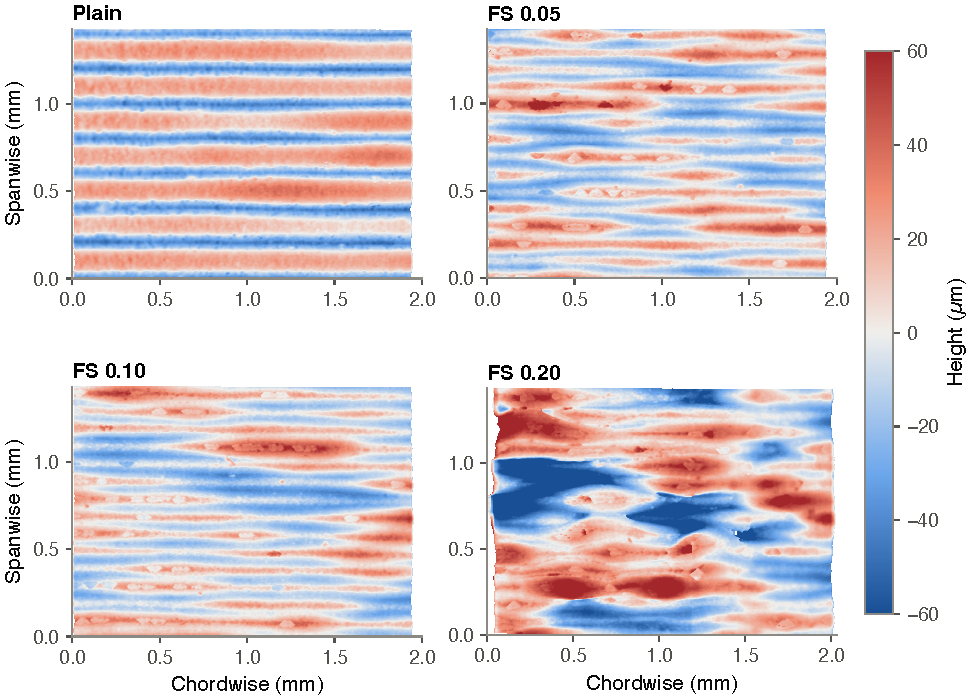
\includegraphics[width=\linewidth]{fig_surface}
  \caption{Profilometer height maps, one field per blade set, each column levelled. Layer lines run
  horizontally (chordwise); profiles for Pa and Ra run vertically (spanwise). Colour clipped at
  $\pm\SI{60}{\micro m}$; FS~0.20 exceeds this over \clipShareC\% of its area.}
  \label{fig:surface}
\end{figure}

% ============================================================== 3 FACILITY ==
\section{Facility and instrumentation}\label{sec:facility}

\subsection{Wind speed}\label{sec:wind}
The tunnel fan is driven by an ABB ACS550 variable-frequency drive, commanded in rpm by a Portenta
Machine Control over Modbus (\figref{fig:rig}). Wind speed $v$ is obtained from the commanded fan
speed $N$ with the tunnel's calibration (Test~1, 13 February 2026), a least-squares line through
\calN{} points (\appref{app:cal}):
\[ v = \calA\,N - \calB \qquad (\si{m/s};\ N \text{ in rpm}). \]
Only \calNmeas{} points were measured, from 0 to \calMeasRpm~rpm (up to \SI{\calMeasV}{m/s}). The
calibration file marks the other \calNtrend, at \calTrendLo--\calTrendHi~rpm, as possibly read from
the trend line of the original record, and the Test~1 instrument is not documented. The \nSPabove{}
set points above \calMeasRpm~rpm (\vAboveLo--\SI{\vHi}{m/s}) therefore rely on air speed remaining
linear in fan speed. At \spLo--\calMeasRpm~rpm the adopted line is \calLowLo--\calLowHi\% above the
measured speeds. A line through the measured points alone gives \SI{\calMeasTop}{m/s} at 1800~rpm,
\calDiffTop\% below the adopted value. This affects absolute wind speeds and $C_{P,\mathrm{el}}$,
not the comparison between rotors, which are compared at identical commanded fan speed.

The median fan-motor current at each set point agreed across the \nRunsWord{} runs within
\SI{\fanRange}{A}, the drive's reading resolution (\SI{\fanTop}{A} at 1800~rpm), so the fan
operating point did not change measurably during the session. Air temperature and pressure were not
recorded. No blockage correction is applied; because the rotors share one geometry, blockage acts on
them alike to first order.

\subsection{Electrical measurement}
The rotor shaft drives a three-phase generator. Its output passes through a three-phase bridge
rectifier to a Chroma 63004-150-60 DC electronic load operated in constant-current mode. A Python
host sets the load current and records the terminal voltage $V$ and current $I$ reported by the
load at the end of each dwell; electrical power is $P=VI$. Every comparison in this report is
between quantities measured with the same instrument at the same settings, so instrument calibration
errors largely cancel. The rig did not log rotor speed; T.~Kang recorded it separately, and every
dwell carries a Unix time stamp for joining that record.

\begin{figure}[h]
  \centering
  % Measurement and control chain used for the rotor sweeps (drawn for this report).
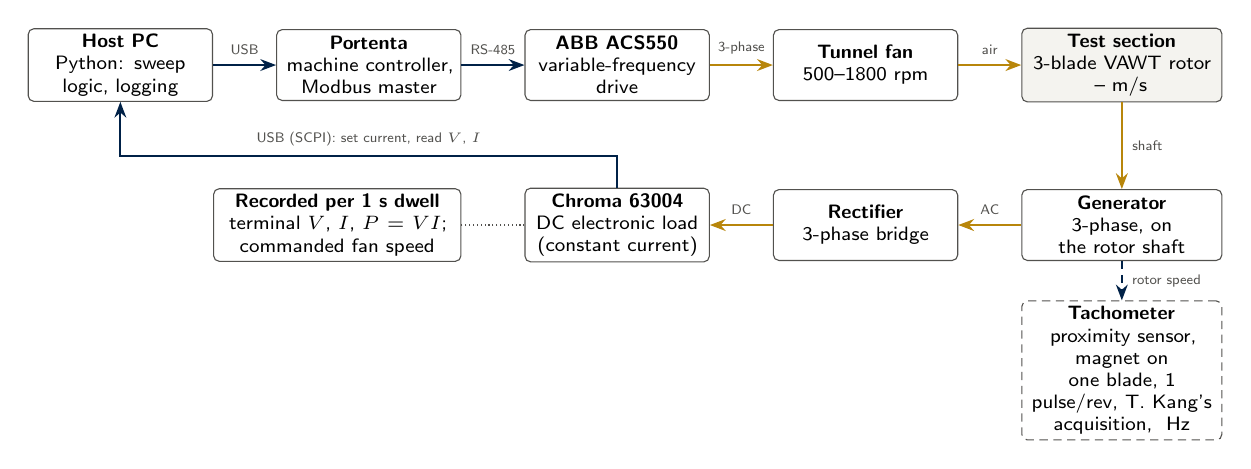
\begin{tikzpicture}[
    font=\sffamily\scriptsize,
    box/.style={draw=ink2, rounded corners=2pt, fill=white, minimum height=9mm,
                text width=22mm, align=center, inner sep=2pt,
                execute at begin node={\hyphenpenalty=10000\exhyphenpenalty=10000}},
    ctl/.style={-{Stealth[length=2mm]}, draw=navy, line width=0.7pt},
    pwr/.style={-{Stealth[length=2mm]}, draw=gold, line width=0.9pt},
    lab/.style={font=\sffamily\tiny, text=ink2},
    node distance=5mm and 8mm]
  % control row
  \node[box] (host) {\textbf{Host PC}\\Python: sweep logic, logging};
  \node[box, right=of host] (pmc) {\textbf{Portenta}\\machine controller, Modbus master};
  \node[box, right=of pmc] (vfd) {\textbf{ABB ACS550}\\variable-frequency drive};
  \node[box, right=of vfd] (fan) {\textbf{Tunnel fan}\\500--1800 rpm};
  \node[box, right=of fan, fill=note, text width=24mm] (ts) {\textbf{Test section}\\3-blade VAWT rotor\\\vLo--\vHi{} m/s};
  % measurement row
  \node[box, below=11mm of ts, text width=24mm] (gen) {\textbf{Generator}\\3-phase, on the rotor shaft};
  \node[box, left=of gen] (rect) {\textbf{Rectifier}\\3-phase bridge};
  \node[box, left=of rect] (load) {\textbf{Chroma 63004}\\DC electronic load (constant current)};
  \node[box, left=of load, text width=30mm] (note) {\textbf{Recorded per 1 s dwell}\\terminal $V$, $I$, $P=VI$;\\commanded fan speed};
  \node[box, below=5mm of gen, text width=24mm, densely dashed] (tach) {\textbf{Tachometer}\\proximity sensor, magnet on one blade, 1 pulse/rev, T.~Kang's acquisition, \tachoFs{} Hz};
  % arrows
  \draw[ctl] (host) -- node[above, lab] {USB} (pmc);
  \draw[ctl] (pmc) -- node[above, lab] {RS-485} (vfd);
  \draw[pwr] (vfd) -- node[above, lab] {3-phase} (fan);
  \draw[pwr] (fan) -- node[above, lab] {air} (ts);
  \draw[pwr] (ts) -- node[right, lab] {shaft} (gen);
  \draw[pwr] (gen) -- node[above, lab] {AC} (rect);
  \draw[pwr] (rect) -- node[above, lab] {DC} (load);
  \draw[ctl] (load.north) |- ++(0,4mm) -| node[pos=0.25, above, lab] {USB (SCPI): set current, read $V$, $I$} (host.south);
  \draw[densely dotted, ink2] (load) -- (note);
  \draw[ctl, densely dashed] (gen) -- node[right, lab] {rotor speed} (tach);
\end{tikzpicture}

  \caption{Measurement and control chain.}
  \label{fig:rig}
\end{figure}

% ============================================================= 4 PROCEDURE ==
\section{Test procedure}\label{sec:procedure}

\subsection{Sweep protocol}
Each run (sweep) visits \nSP{} fan set points from \spLo{} to \spHi~rpm in steps of 100~rpm. At each
set point the host waits until the fan speed is within the larger of \rpmTolAbs~rpm and \rpmTolPct\%
of the command, and then until the generator's terminal voltage has changed by no more than
\settleTolPct\% (and no more than \SI{0.02}{V} where that is larger) over each of \settleConfirm{}
successive \SI{\settlePoll}{s} intervals (at least \SI{\settleMin}{s}; each phase at most
\SI{\settleMax}{s}). The load then raises its current demand in steps of
\SI{\stepmA}{mA} at 1800~rpm (scaled with $v^2$ at lower speeds, minimum \SI{\stepMinmA}{mA}),
dwelling \SI{\dwellS}{s} per step, and stops after \stopConfirm{} consecutive dwells at or below
\stopPct\% of the running maximum. The resulting load ladder of \dwellLo--\dwellHi{} dwells traces
the power--current curve through its maximum (\figref{fig:ladders}). A run takes about \runMin{}
minutes. All runs used the same automated protocol (protocol identifier \texttt{94bed28333f7}).

\begin{figure}[h]
  \centering
  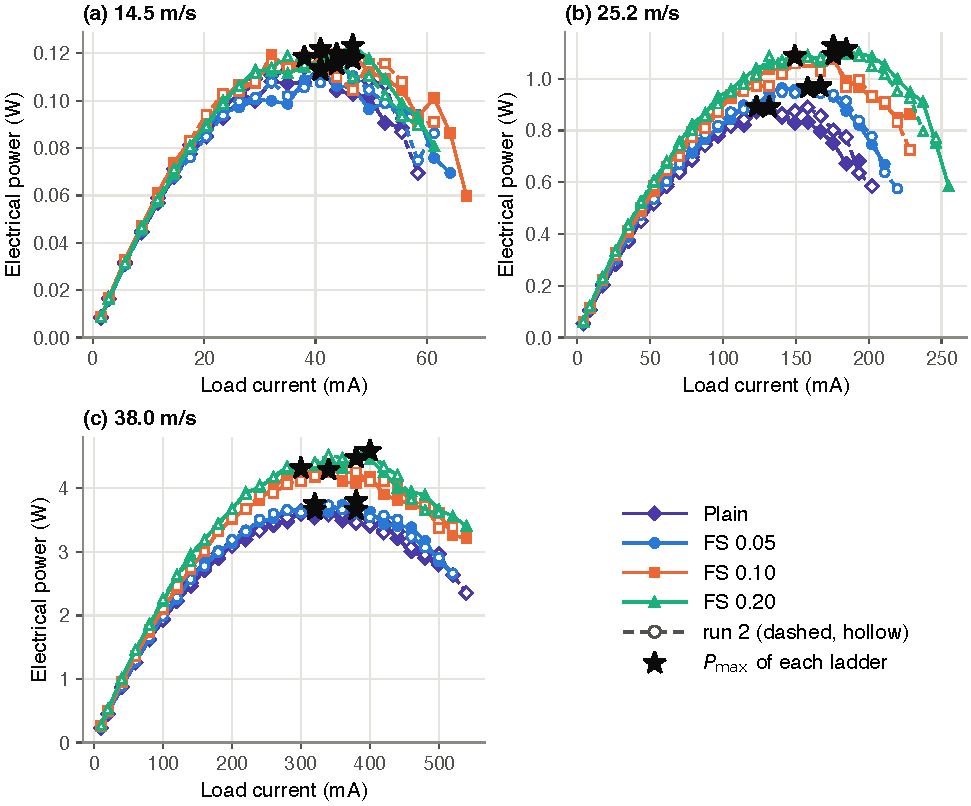
\includegraphics[width=\linewidth]{fig_ladders}
  \caption{Measured load ladders at three wind speeds, all \nRunsWord{} runs (solid: run~1; dashed, hollow:
  run~2). Stars mark $\pmax$, the largest dwell power.}
  \label{fig:ladders}
\end{figure}

\subsection{Session}
Each rotor was mounted once and swept twice without being removed (\tabref{tab:session}), in the
order Plain, FS~0.05, FS~0.10, FS~0.20, from \tFirst{} to \tLast. The two Plain runs started
\plainGap{} minutes apart; the other pairs ran back to back.

\begin{table}[h]
\centering\small
\caption{Runs of 1 October 2026 (local time of the first and last dwell). Change: run mean relative
to the Plain rotor (\secref{sec:stats}).}\label{tab:session}
\begin{tabular}{@{}l c c c l@{}}
\toprule
Rotor & Run & Time & Change (\%) & Data file stem \\
\midrule
\tabinput{../build/tables/session.tex}
\bottomrule
\end{tabular}
\end{table}

\subsection{Data quality}
Of the \nSweeps{} ladders, \nClean{} stopped on the power roll-off. The other \nCut{} stopped on the
load's voltage-floor cut-out after the peak, with the last dwell already below \stopPct\% of the
maximum: \cutList. The peak is therefore inside the ladder in all \nSweeps. Peak powers recomputed
from the dwell records equal the values logged by the rig exactly.

% ============================================================ 5 REDUCTION ==
\section{Data reduction and statistical analysis}\label{sec:stats}

\textbf{Peak power.} $\pmax$ is the largest dwell power in the ladder. As a check, a least-squares
parabola is fitted to the maximum and up to two dwells either side (the rig software's rule); in
\nFallback{} ladders the fit is not concave or its vertex falls outside those dwells, and the maximum is
used. The two estimators give the same conclusions except where noted (\tabref{tab:pairs}). Each
dwell lasts \SI{\dwellS}{s} and rotor speed was not logged, so it is not shown that the rotor reaches
equilibrium within a dwell; at \spLo~rpm it was still accelerating after the settling check
(\tabref{tab:limits}). $\pmax$ is therefore the peak of this ramp protocol.

\textbf{Rotor comparison.} The analysis uses $\ln\pmax$, so differences are ratios. For each run,
$y$ is the mean over the \nSP{} set points of $\ln(\pmax/P_\text{ref})$, where $P_\text{ref}$ is the
geometric mean of the two Plain runs at that set point; each wind speed carries equal weight. The
pooled run-to-run standard deviation of $y$ is $\sigma=\sigRun\%$ (\dofRun{} degrees of freedom).
The rotor effect is tested with a one-way analysis of variance (ANOVA) on the \nRunsWord{} run means, and
all six pairs are compared with Tukey's honestly significant difference procedure, which gives
simultaneous 95\% intervals (family-wise error rate 5\%; studentized range
$q_{0.05;4,\dofRun}=\qTukey$)~\cite{montgomery}. A difference is called resolved when its interval
excludes zero. With two runs per rotor the $p$-values rest on a normal model and are given only down
to 0.001; an exact permutation test of the rotor effect on the \nRunsWord{} run means gives $p=\permP$, the
smallest attainable. Because each rotor's two runs were consecutive, neither test separates a rotor
effect from drift (\secref{sec:limits}).

\textbf{Mounting and drift.} The two runs of a rotor share its print and mounting, so these intervals
measure the repeatability of the measurement on one mounting. Mounting-to-mounting variation $\tau$,
the standard deviation of a rotor's mean power between mountings, was not measured. A difference
stays resolved by the same Tukey criterion for $\tau$ up to \tauPB\% (FS~0.10 vs Plain), \tauPC\% (FS~0.20 vs Plain), \tauAB\% (FS~0.10 vs FS~0.05), \tauAC\% (FS~0.20 vs FS~0.05)
and \tauBC\% (FS~0.20 vs FS~0.10). Because the rotors were run in order of increasing texture, the
run means are also refitted with a linear time term (\secref{sec:limits}).

\textbf{Dependence on wind speed.} A two-way ANOVA with runs nested in rotors tests the rotor $\times$
set point interaction against the residual (run $\times$ set point within rotor), that is, whether
the ratio between rotors changes with wind speed by more than the point-to-point scatter of repeated
runs (\appref{app:stats}). The residual scatter differs between set points, so this $F$ test is
approximate; it is repeated without the two set points with the largest scatter.

\textbf{Source of the gain.} At each set point a straight line $V=V_\mathrm{oc}-IR_\mathrm{int}$, a
Thévenin equivalent, is fitted to the dwells before any cut-out ($r^2\ge\thevRtwo$). $V_\mathrm{oc}$
is its zero-current intercept, an extrapolated open-circuit voltage; for a permanent-magnet generator
it rises in proportion to shaft speed, less a rectifier drop. $R_\mathrm{int}$ is an apparent source
resistance. It includes the winding, rectifier and wiring and the rotor slowing as the load rises;
the latter is large, since a fixed resistance cannot explain the fall from \rintPlainLo\,$\Omega$ at
\SI{\vLo}{m/s} to \rintPlainHi\,$\Omega$ at \SI{\vHi}{m/s} for Plain. $V_\mathrm{oc}^2/4R_\mathrm{int}$ is \matchLo--\matchHi{}
times $\pmax$ over all ladders. Both quantities are compared between rotors as $\pmax$ is.

\textbf{Power coefficient.} The electrical power coefficient is
$C_{P,\mathrm{el}}=\pmax/(\tfrac12\rho A v^3)$ with standard air, $\rho=\SI{\rhoStd}{kg/m^3}$. It
includes generator and rectifier losses and is not the aerodynamic power coefficient. Because
$C_{P,\mathrm{el}}$ is only \cpLo--\cpHi\%, drivetrain losses may be a large share of the power the
rotor extracts, and a fractional change in aerodynamic power can appear magnified in $\pmax$. The
changes reported here are changes in system output.

% =============================================================== 6 RESULTS ==
\section{Results}\label{sec:results}

\subsection{Power curves}
Peak electrical power (rotor means of the two runs) rises from \pLowMin--\SI{\pLowMax}{W} at
\SI{\vLo}{m/s} to \pTopP--\SI{\pTopC}{W} at \SI{\vHi}{m/s} (\figref{fig:power}a). The electrical
power coefficient rises with wind speed for every rotor, from \cpLo\% to \cpHi\%
(\figref{fig:power}b). With the
measured-points-only calibration, $C_{P,\mathrm{el}}$ at \SI{\vHi}{m/s} would be \calCpUnc\% higher
(relative).

\begin{figure}[h]
  \centering
  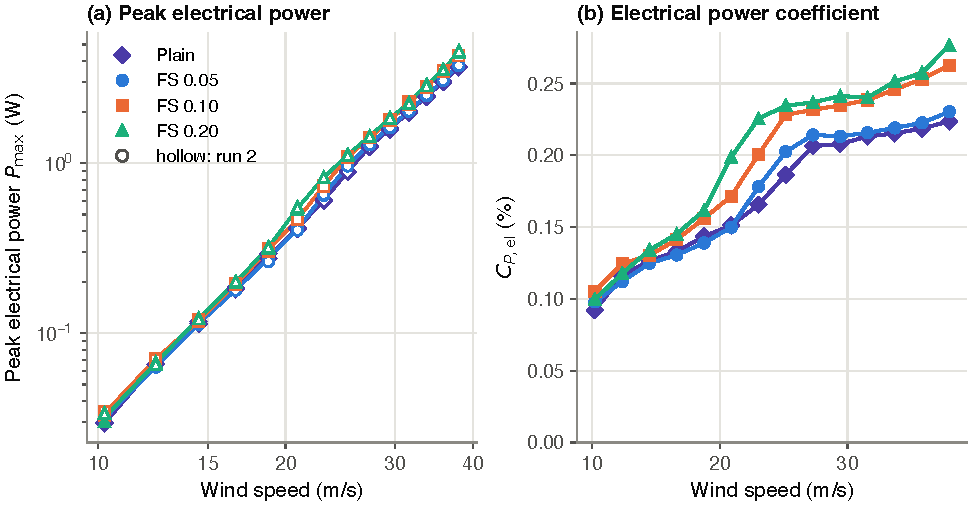
\includegraphics[width=\linewidth]{fig_power}
  \caption{(a) Peak electrical power of every run, logarithmic axes (filled: run~1; hollow: run~2);
  lines join the geometric means of the two runs. (b) Electrical power coefficient, standard air
  density.}
  \label{fig:power}
\end{figure}

\subsection{Rotor comparison}
The rotor effect is large compared with run-to-run variation ($F_{3,\dofRun}=\Frot$,~$p\pRot$;
permutation $p=\permP$). The ratio of the two run means is within \maxPair\% for every rotor
(\figref{fig:runs}), and their scatter is not detectably larger than the point-to-point scatter
within runs ($F_{\dfRunA,\dfRunB}=\Frun$,~$p\pRun$). \nResolvedCap{} of the six pairwise
differences are resolved (\tabref{tab:pairs}); FS~0.05 vs Plain is not. FS~0.20 over FS~0.10 is the
smallest resolved difference; with the parabolic-fit estimator its lower limit is $\fBClo\%$
($p\pfBC$).

\begin{figure}[h]
  \centering
  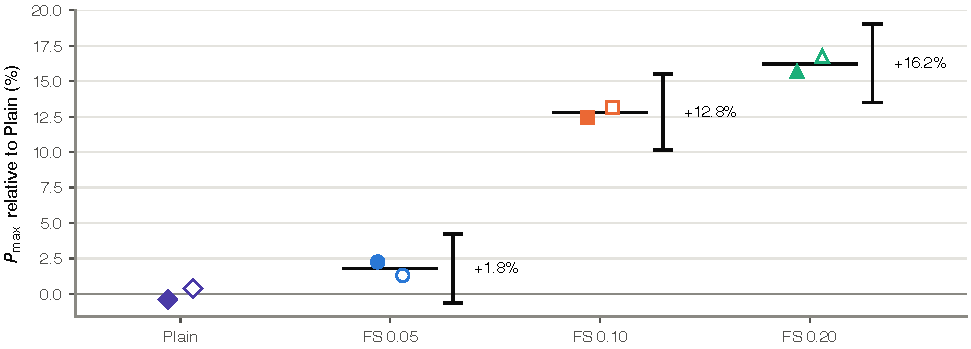
\includegraphics[width=\linewidth]{fig_runs}
  \caption{Each run's mean $\pmax$ relative to the Plain rotor (filled: run~1; hollow: run~2). Bars:
  rotor mean with Tukey simultaneous 95\% interval for the difference from Plain.}
  \label{fig:runs}
\end{figure}

\begin{table}[h]
\centering\small
\caption{Pairwise comparisons of $\pmax$, geometric mean over wind speeds: Tukey simultaneous 95\%
intervals and adjusted $p$-values. Last column: the same for the parabolic-fit
estimator.}\label{tab:pairs}
\begin{tabular}{@{}l c c c c@{}}
\toprule
Comparison & Change (\%) & 95\% CI (\%) & $p$ & Parabolic fit (\%) \\
\midrule
\tabinput{../build/tables/pairs.tex}
\bottomrule
\end{tabular}
\end{table}

\subsection{Dependence on wind speed}
The difference between rotors is not uniform in wind speed (\figref{fig:gain}). The rotor $\times$
set point interaction is large compared with the scatter of repeated runs
($F_{\dfIntA,\dfIntB}=\Fint$,~$p\pInt$). It remains so among the three textured rotors alone
($F_{\dfIntTexA,\dfIntTexB}=\FintTex$,~$p\pIntTex$) and without the two set points with the largest
scatter, \trimDropped~rpm ($F_{\dfIntTrimA,\dfIntTrimB}=\FintTrim$,~$p\pIntTrim$). The steepest
segment of $\ln\pmax$ against $\ln v$, resolved to the \SI{\spDv}{m/s} set-point spacing, lies at
\SI{\stepVC}{m/s} for FS~0.20 and \SI{\stepVB}{m/s} for FS~0.10 in both runs, at
\stepVA\,\si{m/s} for FS~0.05 and at \stepVP\,\si{m/s} for Plain; its slope is \stepSlopeC{} for
FS~0.20 and \stepSlopeP{} for Plain. FS~0.10 and FS~0.20 rise below both Plain runs; FS~0.05 overlaps
Plain. The gains are largest between \bandLo{} and \SI{\bandHi}{m/s}: FS~0.20 exceeds
$+\bandThr\%$ only there, peaking at $\gMaxC\%$ at \SI{\gMaxVC}{m/s}, and FS~0.10 peaks at
$\gMaxB\%$ at \SI{\gMaxVB}{m/s}. Quoted wind speeds
carry the calibration uncertainty of \secref{sec:wind}; the ratios do not.

\begin{figure}[h]
  \centering
  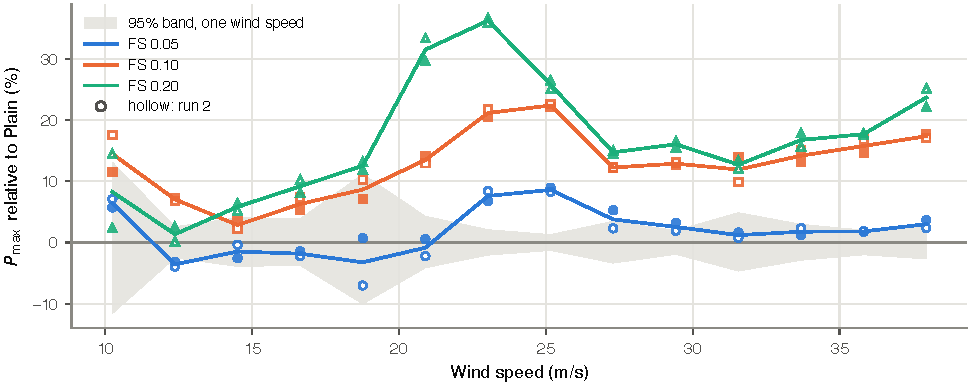
\includegraphics[width=\linewidth]{fig_gain}
  \caption{$\pmax$ of each textured rotor relative to the Plain rotor at each wind speed. Markers:
  individual runs (filled: run~1; hollow: run~2); lines: geometric mean of the two runs. Band: 95\%
  interval of a single-wind-speed difference from run-to-run scatter. All curves share the Plain
  reference, so features common to all three may come from it.}
  \label{fig:gain}
\end{figure}

\subsection{Source of the gain}
Averaged over wind speed, the textured rotors' extrapolated open-circuit voltage is higher than
Plain's, and their source resistance does not differ from it (\tabref{tab:rotor},
\figref{fig:thevenin}). The $V_\mathrm{oc}$ changes alone correspond to power changes of
$\vocSqA\%$, $\vocSqB\%$ and $\vocSqC\%$, against $\cPA\%$, $\cPB\%$ and $\cPC\%$ measured.
$R_\mathrm{int}$ does vary between rotors with wind speed
($F_{\dfIntRintA,\dfIntRintB}=\FintRint$,~$p\pIntRint$): for FS~0.20 it is $\rintMinC\%$ at
\SI{\rintMinVC}{m/s} and $\rintMaxC\%$ at \SI{\rintMaxVC}{m/s} relative to Plain. It is below Plain's
from \rintNegLo{} to \SI{\rintNegHi}{m/s} and above it from \SI{\rintPosLo}{m/s}, a pattern common to
all three textured rotors and so possibly from the Plain reference. Where the gains are largest, the
lower $R_\mathrm{int}$ supplies up to \rintShareMax\% of the gain in $\ln\pmax$. A higher open-circuit
voltage at the same fan speed indicates faster rotation at light load.
Whether this comes from more aerodynamic torque or less parasitic torque cannot be determined from
these data.

\begin{figure}[h]
  \centering
  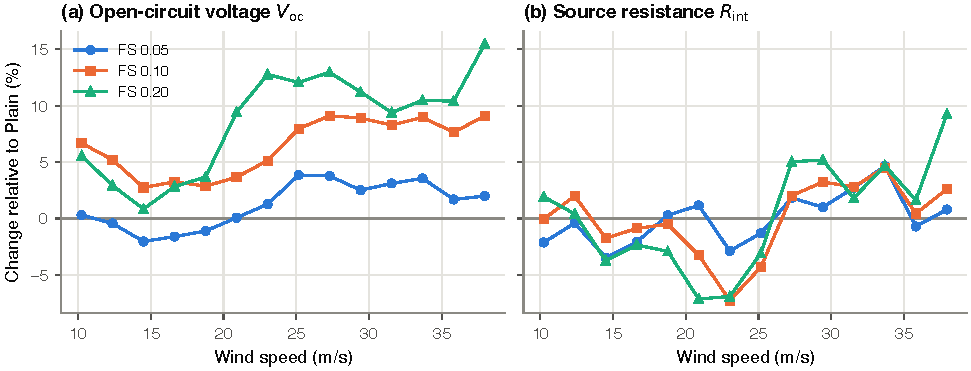
\includegraphics[width=\linewidth]{fig_thevenin}
  \caption{Thévenin decomposition relative to the Plain rotor (geometric mean of two runs).
  (a) Extrapolated open-circuit voltage. (b) Apparent source resistance. All curves share the Plain
  reference, so features common to all three may come from it.}
  \label{fig:thevenin}
\end{figure}

\begin{table}[h]
\centering\small
\caption{Thévenin parameters relative to Plain, mean over wind speeds, with Tukey simultaneous 95\%
intervals; electrical power coefficient at \vHi\,m/s, standard air.}\label{tab:rotor}
\begin{tabular}{@{}l c c c@{}}
\toprule
Rotor & $V_\mathrm{oc}$ (\%) & $R_\mathrm{int}$ (\%) & $C_{P,\mathrm{el}}$ (\%) \\
\midrule
\tabinput{../build/tables/rotor.tex}
\bottomrule
\end{tabular}
\end{table}

\subsection{Surface roughness and power}
The measured surface parameters do not order the rotors as their power does
(\tabref{tab:headline}). Ra is highest on Plain, from its layer lines, and ranks FS~0.05 above
FS~0.10; the textured sets span \RaB--\RaC\,\si{\micro m}, about the \RaSpreadC\,\si{\micro m} by
which the two FS~0.20 fields differ. Pa ranks FS~0.20 highest and Plain second, and does not separate
FS~0.05 from FS~0.10, although their power differs by $\cAB\%$: either the realised texture of these
two sets does not follow the setting, or one field per set does not resolve it. The power ranking
matches the nominal fuzzy-skin thickness; with one print per level this is an association
(\secref{sec:limits}).

% ================================================================ 7 LIMITS ==
\section{Uncertainty and limitations}\label{sec:limits}

\tabref{tab:limits} lists the sources of uncertainty. Two are not covered by the intervals.
\begin{itemize}
  \item \textbf{Print and mounting.} Each texture level is one print mounted once, so print-to-print
        and mounting variation are confounded with texture; \secref{sec:stats} gives the mounting
        variation each difference could absorb. The Plain set also differs in layer height
        (\SI{0.2}{mm} against about \SI{0.1}{mm}), and its printer, nozzle and material are unknown.
        FS~0.05 and FS~0.10 share a \SI{\pitchA}{mm} layer period, so their difference ($\cAB\%$
        $[\cABlo,\ \cABhi]$) is the comparison least affected by layer height.
  \item \textbf{Run order.} The rotors were run in order of increasing texture, so slow drift is
        confounded with texture. A fit of the \nRunsWord{} run means with a rotor term and a linear time
        term gives a drift of $\driftRate\%$ per hour (95\% interval $\driftLo\%$ to $\driftHi\%$).
        With that term, FS~0.10 and FS~0.20 remain resolved from Plain ($\cdB\%$ $[\cdBlo,\ \cdBhi]$
        and $\cdC\%$ $[\cdClo,\ \cdChi]$; $t$ intervals, \driftDof{} degrees of freedom), while
        FS~0.05 is $\cdA\%$ $[\cdAlo,\ \cdAhi]$. A linear drift of this size cannot explain the
        FS~0.10 and FS~0.20 differences but could account for the FS~0.05 difference; a change that
        occurred between rotors, rather than steadily, cannot be separated from a rotor effect with
        these data.
\end{itemize}

\begin{table}[h]
\centering\small
\caption{Sources of uncertainty.}\label{tab:limits}
\begin{tabularx}{\linewidth}{@{}>{\raggedright}p{0.21\linewidth} >{\raggedright}p{0.3\linewidth} X@{}}
\toprule
Source & Size & Effect on the rotor comparison \\
\midrule
Run-to-run repeatability & $\sigma=\sigRun\%$ (run mean); \sigE\% per point & In every interval. \\
Peak estimator & Changes within \fitMaxDiff{} percentage points & FS~0.20 vs FS~0.10 becomes marginal (\tabref{tab:pairs}). \\
Drift during the session & $\driftRate\%$/h $[\driftLo,\ \driftHi]$ & Confounded with run order; a linear-drift fit leaves FS~0.10 and FS~0.20 resolved. \\
Ramp dynamics & \SI{\dwellS}{s} dwells, equilibrium not verified; at \spLo~rpm the voltage rose between the first two dwells in \nRise{} of \nRunsWord{} runs & Common protocol, but a bias that depends on rotor inertia or torque--speed slope would not cancel. \\
Wind-speed calibration & \calLowLo--\calLowHi\% high at \calLowVLo--\SI{\calLowVHi}{m/s}; \calDiffTop\% above a line through the measured points only at \SI{\vHi}{m/s} (an extrapolation, not a bound) & None on the comparison (identical fan speeds); affects absolute $v$ and $C_{P,\mathrm{el}}$. \\
Air density & Not recorded & Any change is confounded with run order (see drift); $C_{P,\mathrm{el}}$ assumes standard air. \\
Blockage & Not corrected & Similar for rotors of one geometry; not quantified (test-section size not documented). \\
Electrical measurement & Not quantified & Largely cancels (same instrument and settings). \\
Print and mounting & Not measured & Not in the intervals; \secref{sec:stats} gives the variation each difference can absorb. \\
\bottomrule
\end{tabularx}
\end{table}

% =========================================================== 8 CONCLUSIONS ==
\section{Conclusions}\label{sec:conclusions}
\begin{enumerate}
  \item On 1 October 2026 the FS~0.10 and FS~0.20 rotors produced $\cPB\%$ $[\cPBlo,\ \cPBhi]$ and
        $\cPC\%$ $[\cPClo,\ \cPChi]$ more peak electrical power than the Plain rotor, averaged over
        \vLo--\vHi\,\si{m/s}. The FS~0.05 difference, $\cPA\%$ $[\cPAlo,\ \cPAhi]$, was not resolved
        and could be produced by session drift.
  \item The advantage varies with wind speed: the power coefficient of FS~0.10 and FS~0.20 rises
        more steeply, and at lower wind speed, than Plain's, so the gains are largest at
        \bandLo--\SI{\bandHi}{m/s}.
  \item Averaged over wind speed, the gain is carried by the extrapolated open-circuit voltage,
        which indicates faster rotation of the textured rotors at light load; where the gains are
        largest, a lower apparent source resistance also contributes.
  \item Ra and Pa, as scanned (one field per set), do not order the rotors by power: FS~0.05 and
        FS~0.10 have similar Pa but differ by $\cAB\%$ in power, so the scans do not confirm that
        their realised texture differs.
  \item The intervals reflect run-to-run repeatability on one print and one mounting per texture.
        The FS~0.10 and FS~0.20 differences from Plain would stay resolved with mounting variation of
        up to about \tauPB--\tauPC\% (Tukey criterion); replicate prints and mountings are needed to
        measure that variation and to attribute the differences to texture.
\end{enumerate}

% ================================================================== 9 NEXT ==
\section{Recommendations}\label{sec:next}
\begin{enumerate}
  \item \textbf{Replicate and randomise.} Print at least two sets per thickness, including a Plain set
        at the textured sets' \SI{0.1}{mm} layer height. Mount each set twice and run in an
        interleaved order, re-running the Plain reference after every third rotor. This measures
        print and mounting variation and removes the run-order confound.
  \item \textbf{Add rotor speed.} Join T.~Kang's rotor-speed record to the dwells to obtain tip-speed
        ratio $\lambda$ and $C_{P,\mathrm{el}}(\lambda)$. Separating aerodynamic from parasitic torque
        also needs a spin-down or motored friction test of each mounted rotor.
  \item \textbf{Extend the wind calibration} with a direct air-speed measurement over the test range;
        record air temperature and pressure on every run; document the test-section dimensions for
        a blockage estimate.
  \item \textbf{Characterise the surfaces at fixed stations}: several fields per set on two blades
        and both faces, profiles along and across the layer lines, and an evaluation length of at
        least five cut-off lengths. Keep the sliced file, printer, nozzle and filament record for
        every print.
\end{enumerate}

\subsection{Toward the fault-testing plan}\label{sec:faults}
Prof.\ Jeong asked for a fault-testing plan agreed before the next round. The rig offers an automated
sweep of about \runMin{} minutes with run-to-run repeatability of \sigRun\% (run mean; repeat runs
on one mounting, back to back except Plain's, \plainGap{} minutes apart). Whether $V_\mathrm{oc}$ and $R_\mathrm{int}$ separate rotor-side from
electrical faults is untested: $R_\mathrm{int}$ also reflects the rotor slowing under load
(\secref{sec:stats}), so this should be checked on the first fault cases together with rotor speed.
Candidate faults are a tip mass on one blade (imbalance); a chipped, shortened or missing blade;
added bearing drag; and an open or high-resistance generator phase. A short meeting to agree the
fault list, severity levels and acceptance criteria should precede any fault prints.

\section*{Acknowledgement}
T.~Kang provided the electronic load and recorded rotor speed during the session.

\begin{thebibliography}{9}
\bibitem{iso16610} ISO 16610-21:2011, \emph{Geometrical product specifications (GPS) --- Filtration
--- Part 21: Linear profile filters: Gaussian filters}.
\bibitem{montgomery} D.~C. Montgomery, \emph{Design and Analysis of Experiments}, 9th ed., Wiley,
2017.
\bibitem{iso4288} ISO 4288:1996, \emph{Geometrical product specifications (GPS) --- Surface texture:
Profile method --- Rules and procedures for the assessment of surface texture}; superseded by
ISO 21920-3:2021.
\end{thebibliography}

% ============================================================= APPENDICES ==
\appendix

\section{Peak power by run and set point}\label{app:data}
\begin{table}[h]
\centering\footnotesize
\caption{Peak electrical power $\pmax$ (W), largest dwell, every run. Runs 1 and 2 share the rotor's
mounting.}\label{tab:data}
\setlength{\tabcolsep}{4pt}
\begin{tabular}{@{}rr rr rr rr rr@{}}
\toprule
Fan & $v$ & \multicolumn{2}{c}{Plain} & \multicolumn{2}{c}{FS 0.05} & \multicolumn{2}{c}{FS 0.10} & \multicolumn{2}{c}{FS 0.20} \\
\cmidrule(lr){3-4}\cmidrule(lr){5-6}\cmidrule(lr){7-8}\cmidrule(lr){9-10}
rpm & m/s & 1 & 2 & 1 & 2 & 1 & 2 & 1 & 2 \\
\midrule
500 & 10.2 & 0.0294 & 0.0298 & 0.0313 & 0.0317 & 0.0330 & 0.0348 & 0.0303 & 0.0339 \\
600 & 12.4 & 0.0658 & 0.0660 & 0.0638 & 0.0633 & 0.0707 & 0.0704 & 0.0676 & 0.0660 \\
700 & 14.5 & 0.1140 & 0.1175 & 0.1128 & 0.1153 & 0.1197 & 0.1184 & 0.1232 & 0.1218 \\
800 & 16.6 & 0.1858 & 0.1811 & 0.1808 & 0.1794 & 0.1931 & 0.1969 & 0.1983 & 0.2023 \\
900 & 18.8 & 0.2753 & 0.2937 & 0.2864 & 0.2644 & 0.3045 & 0.3135 & 0.3181 & 0.3220 \\
1000 & 20.9 & 0.4162 & 0.4109 & 0.4158 & 0.4044 & 0.4716 & 0.4671 & 0.5362 & 0.5516 \\
1100 & 23.0 & 0.6093 & 0.6031 & 0.6474 & 0.6572 & 0.7309 & 0.7381 & 0.8278 & 0.8240 \\
1200 & 25.2 & 0.8894 & 0.8914 & 0.9700 & 0.9642 & 1.0875 & 1.0921 & 1.1261 & 1.1142 \\
1300 & 27.3 & 1.2706 & 1.2463 & 1.3247 & 1.2875 & 1.4130 & 1.4123 & 1.4403 & 1.4474 \\
1400 & 29.4 & 1.5788 & 1.5975 & 1.6391 & 1.6184 & 1.7898 & 1.7959 & 1.8351 & 1.8511 \\
1500 & 31.6 & 1.9799 & 2.0368 & 2.0413 & 2.0236 & 2.2892 & 2.2066 & 2.2762 & 2.2513 \\
1600 & 33.7 & 2.4530 & 2.4832 & 2.4978 & 2.5259 & 2.7952 & 2.8414 & 2.9085 & 2.8549 \\
1700 & 35.8 & 3.0003 & 3.0273 & 3.0671 & 3.0700 & 3.4574 & 3.5213 & 3.5436 & 3.5516 \\
1800 & 38.0 & 3.6640 & 3.6666 & 3.7998 & 3.7517 & 4.3137 & 4.2905 & 4.4798 & 4.5882 \\
\bottomrule
\end{tabular}

\end{table}

\section{Statistical details}\label{app:stats}
\textbf{Model.} With $y_{rjs}=\ln\pmax$ for rotor $r$ (4), run $j$ (2) and set point $s$ (14),
\[ y_{rjs} = \mu + \alpha_r + \beta_s + (\alpha\beta)_{rs} + u_{rj} + e_{rjs}, \]
where $u_{rj}$ is a run offset within the rotor and $e_{rjs}$ the residual~\cite{montgomery}. The
rotor effect is tested against run within rotor, which is the one-way ANOVA on run means. The
interaction $(\alpha\beta)_{rs}$ and the run term are tested against the residual
(\tabref{tab:anova}). Run offsets do not enter either mean square, so the interaction test needs no
assumption about them; it does assume equal residual variance, so it is approximate here.

\begin{table}[h]
\centering\small
\caption{Analysis of variance of $\ln\pmax$. MS in units of $10^{-4}$.}\label{tab:anova}
\begin{tabular}{@{}l r r r r l@{}}
\toprule
Source & df & MS & $F$ & $p$ & Tested against \\
\midrule
\tabinput{../build/tables/anova.tex}
\bottomrule
\end{tabular}
\end{table}

\textbf{Comparisons.} With run means $\bar y_{rj}$, rotor means $\bar y_r$ and pooled
$\sigma^2=\sum_r\sum_j(\bar y_{rj}-\bar y_r)^2/4$, Tukey's interval for rotors $a$ and $b$ is
$\exp\!\big(\bar y_b-\bar y_a \pm q_{0.05;4,4}\,\sigma/\sqrt2\big)-1$, a half-width of \hwTukeyLog{}
in $\ln\pmax$ (about \hwTukey\%). The same procedure is applied to $\ln V_\mathrm{oc}$ and
$\ln R_\mathrm{int}$. The permutation test enumerates all \permN{} ways of splitting the \nRunsWord{} run
means into four pairs.

\textbf{Mounting variation.} If each rotor's mean carried an independent mounting offset with
standard deviation $\tau$, the difference of two rotor means would have variance $\sigma^2+2\tau^2$.
It stays resolved by the Tukey criterion while
$|\bar y_b-\bar y_a|>(q_{0.05;4,4}/\sqrt2)\sqrt{\sigma^2+2\tau^2}$, which gives the values of $\tau$
quoted in \secref{sec:stats}.

\textbf{Drift.} The run means are fitted as $\bar y_{rj}=a_r+\beta t_{rj}$, with $t_{rj}$ the start
time of the run in hours, by least squares (\driftDof{} residual degrees of freedom).

\textbf{Residual scatter.} The per-point residual standard deviation is \sigE\% overall; it is largest
at \sigEmaxRpm~rpm (\sigEmax\%) and smallest at \sigEminRpm~rpm (\sigEmin\%).

\section{Surface analysis}\label{app:surface}
The Keyence export is a height map in millimetres, quantised to \SI{1}{\micro m}. Each image column is
one spanwise profile. A column is dropped if more than 10\% of its points are missing, or if more than
2\% are missing between its first and last valid points (\rejLo\% of columns or fewer for Plain,
FS~0.05 and FS~0.10; \rejC\% for FS~0.20, where missing points concentrate on steep slopes, so its
values may be slightly low). The remaining interior gaps are filled linearly, a least-squares line is
removed, and the profiles of a field are cut to the length of the shortest one. Pa is the mean
absolute deviation of the levelled profile. For Ra the levelled profile minus its ISO~16610-21
Gaussian mean line ($\alpha=\sqrt{\ln2/\pi}$, $\lambda_c=\SI{0.25}{mm}$) is evaluated with $\lambda_c/2$
discarded at each end~\cite{iso16610}. The layer period is the peak of the mean power spectrum between
60 and \SI{320}{\micro m}. For periodic profiles ISO~4288~\cite{iso4288} selects
$\lambda_c=\SI{0.25}{mm}$ for spacings of 0.04--\SI{0.13}{mm}, which fits FS~0.05 and FS~0.10. The
Plain set's \SI{0.2}{mm} period would call for \SI{0.8}{mm}, and the non-periodic FS~0.20 surface (Ra
above \SI{10}{\micro m}) for \SI{8}{mm}, both longer than the \fieldY\,mm field. The filter transmits
50\% at $\lambda_c$: Ra keeps about \transP\% of the amplitude of the Plain set's \SI{\pitchP}{mm} layer
lines and \transA\% of the \SI{\pitchA}{mm} ones, so Plain's Ra is understated relative to FS~0.05 and
FS~0.10. Pa is unfiltered.

\section{Wind-speed calibration}\label{app:cal}
\begin{figure}[h]
  \centering
  \begin{minipage}[t]{0.6\linewidth}\vspace{0pt}
    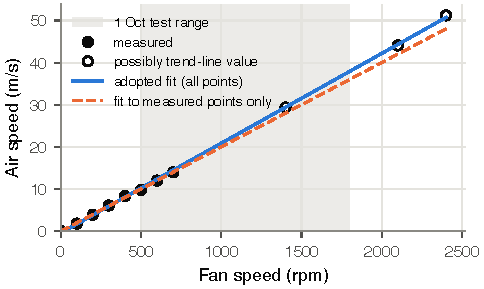
\includegraphics[width=\linewidth]{fig_calibration}
  \end{minipage}\hfill
  \begin{minipage}[t]{0.37\linewidth}\vspace{4pt}
  \caption{Tunnel calibration, Test~1 (13 February 2026). Filled: measured; hollow: marked in the
  calibration file as possibly read from the trend line of the original record. Shaded: the range of
  this test.}
  \label{fig:cal}
  \end{minipage}
\end{figure}
\begin{table}[h]
\centering\small
\caption{Calibration points and the adopted fit $v=\calA N-\calB$ (\figref{fig:cal}). A line through
the measured points alone has residual standard deviation \SI{\calMeasSd}{m/s}.}\label{tab:cal}
\begin{tabular}{@{}r r l r r@{}}
\toprule
Fan (rpm) & $v$ (m/s) & Source & Fit (m/s) & Fit $-$ measured (m/s) \\
\midrule
\tabinput{../build/tables/calibration.tex}
\bottomrule
\end{tabular}
\end{table}

\section{Data package and reproducibility}\label{app:package}
The accompanying archive contains:
\begin{itemize}
  \item \texttt{1\_rig\_sweeps/}: the raw files of the \nRunsWord{} runs;
  \item \texttt{2\_surface\_scans/}: the profilometer height maps;
  \item \texttt{3\_derived/}: the analysis-ready tables behind this report;
  \item \texttt{4\_reference/}: the rotor geometry, blade mesh, wind calibration and slicer summary;
  \item \texttt{5\_figures/} and \texttt{6\_code/}: the figures and the analysis code.
\end{itemize}
\texttt{README.md} explains the layout, \texttt{DATA\_DICTIONARY.md} defines every column, and
\texttt{MANIFEST.csv} gives each file's SHA-256 checksum. The script
\texttt{6\_code/build\_report.py} (Python~3) regenerates every result, table and data figure in this
report from the raw files.

\end{document}
